\chapter{実装}
\label{chap:implementation}

本研究では、\ref{chap:design}章で示した設計のうち、WebAssemblyプログラムの実行部分に着目し、その実現可能性を評価するため、マイコン上にWebAssembly実行環境を実装した。

ハードウェアには、TCPやHTTPが実装可能な性能を持つマイコンとして、Espressif SystemsのESP32\cite{esp32}を用いた。

本章では、ESP32上に実装した実行環境の構成と、WebAssemblyバイナリの実行フローについて述べる。

\section{全体の構成}

本実装の構成を図\ref{fig:esp32_libwasm}に示す。
本実装は、C言語で実装したWebAssemblyバイナリのインタプリタ(libwasm)と、libwasmが提供する機能を呼び出すESP32用のプログラム(ホストプログラム)より構成される。
HTTPサーバとの通信部分は実装せず、実行するWebAssemblyバイナリは静的にホストプログラムに埋め込んだ。

ホストプログラムは、libwasmを用いてWebAssemblyバイナリが定義するモジュールを読み込み、モジュールが持つ関数を呼び出し、結果を標準出力に表示する。

なお、実装の簡便のため、モジュールの検証は実装しなかった。
また、設計上複数モジュールの実行は想定していないため、インポートおよびエクスポートに関する機能は実装しなかった。
命令セットについては、仕様が定義する172命令のうち、\ref{chap:evaluation}章で述べる検証用プログラムの実行に必要な16命令のみを実装した。

\begin{figure}[htbp]
  \caption{本実装の構成}
  \label{fig:esp32_libwasm}
  \begin{center}
    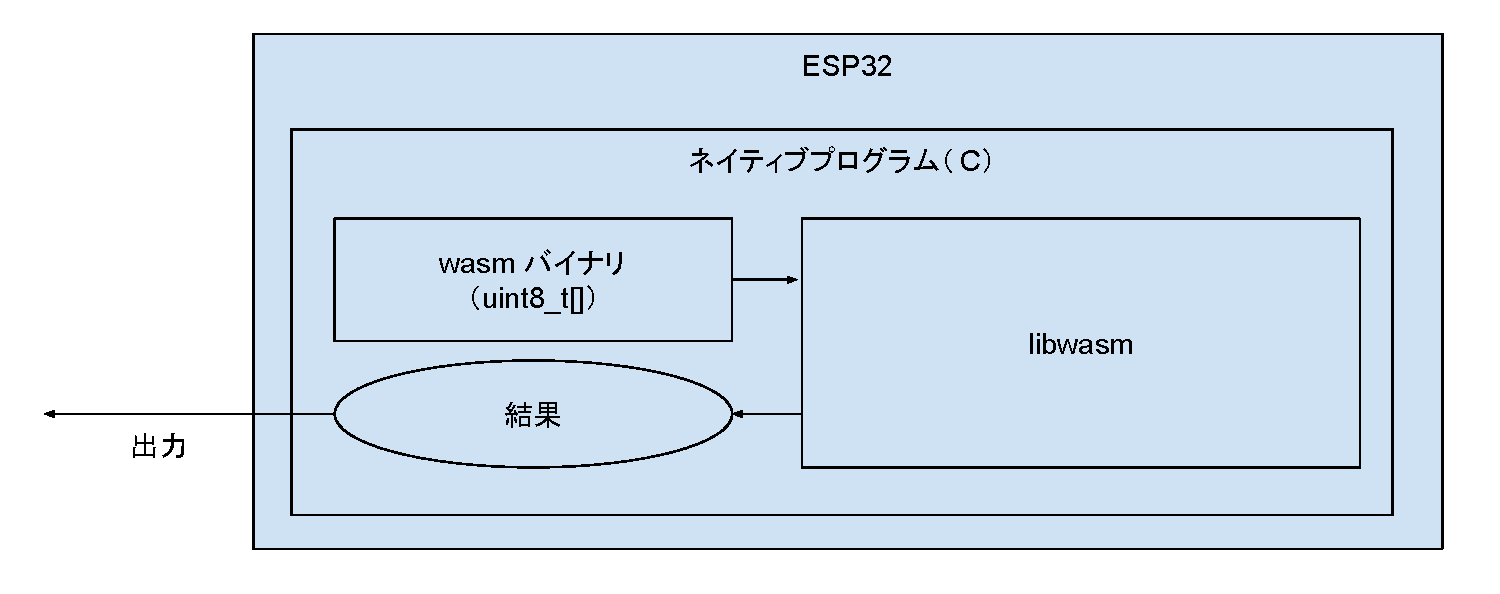
\includegraphics[bb=0 0 720 285,width=12cm]{img/esp32_libwasm.pdf}
  \end{center}
\end{figure}

\section{WebAssembly実行環境}

WebAssembly Core Specification\cite{wasm_spec}により規定された仕様を基に、WebAssemblyインタプリタをライブラリ「libwasm」としてC言語により実装した。
libwasmはC11により標準化された仕様のみを用いてプラットフォーム非依存な形で実装したため、ESP32以外のマイコンにも容易に移植可能であると考えられる。

libwasmは、主に以下の三つの機能を提供する:

\begin{itemize}
  \item バイナリをWebAssemblyモジュールとしてパースする
  \item パースして得られたWebAssemblyモジュールを実行可能な形式にインスタンス化する
  \item インスタンス化したモジュールが持つ関数を呼び出し、結果を得る
\end{itemize}

libwasmの動作概観を\ref{fig:libwasm_arch}に示す。

\begin{figure}[htbp]
  \caption{libwasmの動作概観}
  \label{fig:libwasm_arch}
  \begin{center}
    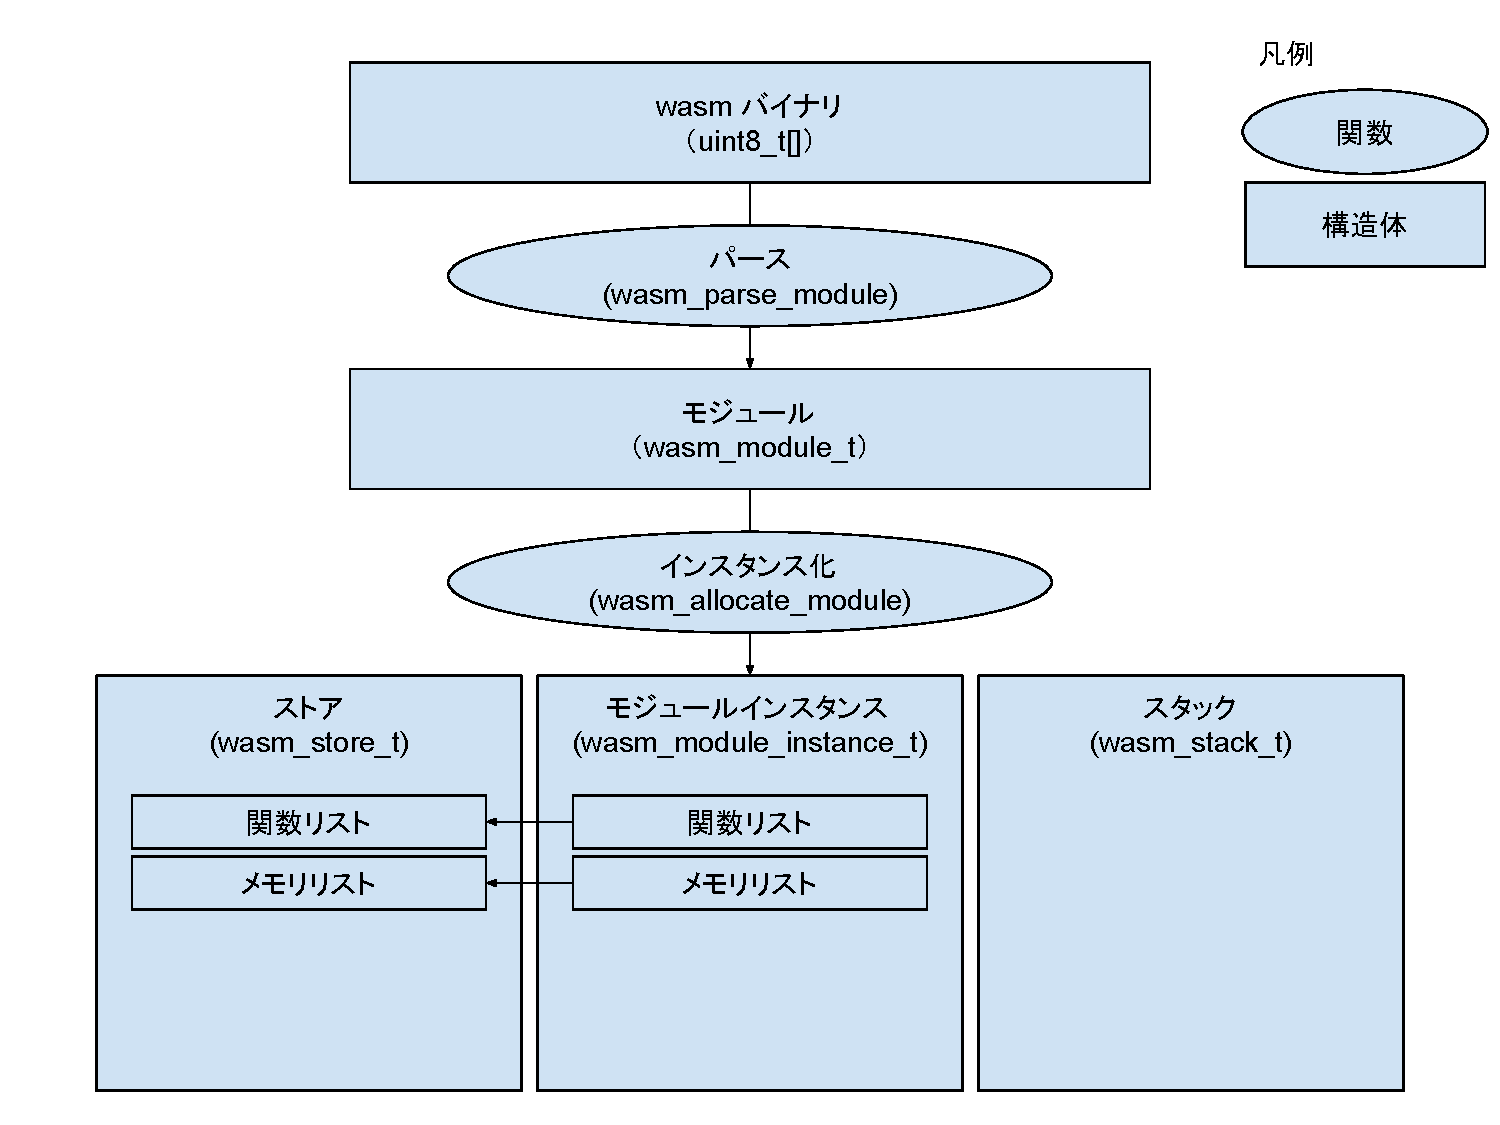
\includegraphics[bb=0 0 915 667,width=15cm]{img/libwasm_arch.pdf}
  \end{center}
\end{figure}

\subsection{パース}

\subsubsection{モジュール}

\verb|wasm_parse_module|関数は、バイト列として表現されたWebAssemblyバイナリを再帰下降構文解析によりパースし、\verb|wasm_module_t|構造体として表現されたWebAssemblyモジュールを生成する。

WebAssemblyバイナリは、4バイトのマジックナンバー{\tt 0x00 0x61 0x73 0x6D}(\verb*| asm|)、4バイトのバージョン番号、そして連続した{\bf セクション}の列として表現される。
\verb|wasm_parse_module|関数は、マジックナンバーおよびバージョン番号(本実装では定数{\tt 0x01 0x00 0x00 0x00})を解釈した後、各セクションをパースする。

\subsubsection{セクション}

WebAssemblyモジュールは、10種の{\bf 定義済みセクション}と、コンパイラやユーザが自由に用途を決められる{\bf カスタムセクション}を持つ。
各セクションはIDを持ち、10種の定義済みセクションはそれぞれ一つのモジュール内で一度のみ、IDが昇順になる順番で現れる。
ただし、カスタムセクションは数および場所を問わず現れることができる。

セクションの一覧を表\ref{tb:wasm_sections}に示す。

\begin{table}[htbp]
  \begin{center}
    \caption{WebAssemblyモジュールにおけるセクションの一覧}
    \label{tb:wasm_sections}
    \begin{tabular}{|c|l|l|}
      \hline
      セクションID & セクションの種類 \\\hline\hline
      0 & カスタムセクション \\\hline
      1 & 型セクション \\\hline
      2 & インポートセクション \\\hline
      3 & 関数セクション \\\hline
      4 & テーブルセクション \\\hline
      5 & メモリセクション \\\hline
      6 & グローバルセクション \\\hline
      7 & エクスポートセクション \\\hline
      8 & 開始セクション \\\hline
      9 & エレメントセクション \\\hline
      10 & コードセクション \\\hline
      11 & データセクション \\\hline
    \end{tabular}
  \end{center}
\end{table}

各セクションは、セクションIDとセクションのバイト数から始まり、それぞれのセクション固有の情報が続く。\verb|wasm_parse_module|関数は、セクションの先頭のIDを読み、それぞれのセクションをパースする関数(\verb|wasm_parse_custom_section|、\verb|wasm_parse_type_section|など)を呼び出す。

\subsubsection{値}

整数は、{\bf LEB128}により表現される。LEB128はデバッグファイルフォーマットのDWARFでも用いられている\cite{dwarf}整数の可変長バイナリ表現であり、値が小さい場合に効率的に表現できる。

浮動小数点数はIEEE 754-2008\cite{ieee754}に従い、リトルエンディアンで表現される。

LEB128で表現された整数、IEEE 754に従って表現された浮動小数点数のそれぞれについて、パーサを実装した。

% \subsubsection{型}

% WebAssemblyは32ビットおよび64ビット整数、32ビットおよび64ビット浮動小数点数の4種類の型が用意されている。

% \subsubsection{コード}

\subsection{インスタンス化}

\verb|wasm_parse_module|関数により得られたモジュールは、WebAssemblyプログラムの情報を格納したものであり、プログラムの実体ではない。
そこで、モジュールを実行可能な形式に実体化するために、モジュールの{\bf インスタンス化}を行う必要がある。

モジュールをインスタンス化することにより、モジュールの関数セクション、テーブルセクション、メモリ、グローバルの情報に基づいて、それぞれ関数インスタンス、テーブルインスタンス、メモリインスタンス、グローバルインスタンスが作成される。

各インスタンスは、\verb|wasm_store_t|構造体で表現されるストアに格納される({\bf アロケーション})。
同じストアを用いて複数のモジュールをインスタンス化することも可能であり、各インスタンスは全てのモジュールの中で一意な整数のアドレスが付与される。
\verb|wasm_allocate_module|関数が最終的に返す\verb|wasm_module_instance_t|は、各インスタンスのアドレスのリストのみを持つ。

\subsubsection{関数インスタンス}

\verb|wasm_function_instance_t|構造体で表現される関数インスタンスは、関数の型、実行内容を表す命令列({\bf コード})、およびその関数が定義されているモジュールインスタンスへの参照を持つ。

\subsubsection{テーブルインスタンス}

\verb|wasm_table_instance_t|構造体で表現されるテーブルインスタンスは、関数アドレスのリストを持つ。

\subsubsection{メモリインスタンス}

\verb|wasm_memory_instance_t|構造体で表現されるメモリインスタンスは、バイト単位でアクセス可能なデータ領域を8ビット整数の配列として持つ。また、必要に応じてデータ領域の最大サイズを持つ。

\subsubsection{グローバルインスタンス}

\verb|wasm_global_instance_t|構造体で表現されるグローバルインスタンスは、グローバル変数として用いられる値のリストを持つ。

テーブルインスタンス、メモリインスタンスおよびグローバルインスタンスは、それぞれモジュールのエレメントセクション、データセクション、グローバルセクションで指定された値によって初期化される。

モジュールに格納された各情報に対応した全てのインスタンスがストアにアロケートされた後、モジュールに開始セクションがある場合は、開始セクションにより指定された関数がエントリーポイントとして呼び出される。

\subsection{スタック}

WebAssemblyにおける関数の実行は、全ての命令が\verb|wasm_stack_t|構造体で表現される{\bf スタック}を対象するスタックマシンとして定義されている。
スタックには、命令のオペランドとなる値、ループ命令や分岐命令といった制御命令の対象となる{\bf ラベル}、関数の呼び出しおよびリターン時に用いられる{\bf フレーム}(または{\bf アクティベーション})が要素として格納される。

WebAssemblyにおけるスタックはプッシュおよびポップ以外の操作で変更されることはなく、値が参照されるのは先頭の要素のみであるため、連続したメモリ空間に配置する必要がない。そのため、本実装では線形リストとして実装した。

\subsubsection{値}
値は\verb|wasm_value_t|構造体で定義される。

型情報(i32,i64,f32,f64)と実際の値を持つ。

\subsubsection{ラベル}
\verb|wasm_label_t|構造体。

arityと継続(continuation)を持つ。

\subsubsection{フレーム}
\verb|wasm_frame_t|構造体。

arity、ローカル変数のリスト、モジュールインスタンスへの参照を持つ。

\subsection{モジュール外部からの関数呼び出し}

モジュールのインスタンス化が完了した後、関数インスタンスに対応するアドレスを指定することで該当する関数を呼び出すことができる。

モジュールインスタンスの関数を呼び出す際は、\verb|wasm_invoke|関数にストア、スタック、モジュールインスタンス、関数アドレス、引数となる値をリストとして与える。\verb|wasm_invoke|関数は、与えられた引数のリストが含む値を全てスタックにプッシュした後、モジュール内部からの呼び出しとして関数を実行する。

\subsection{モジュール内部からの関数呼び出し}

関数が呼び出された際、関数が引数として取る値の数だけスタックから値をポップし、これらの値を持ったフレームを作成する。このフレームをスタックにプッシュしたのち、関数が持つコードを\verb|block|命令として実行する。

\subsection{各命令の実行}

\subsubsection{{\tt block} 命令、 {\tt loop} 命令}

引数として命令のリストを持ち、ブロックの実行を始める。

スタックにフレームを積んだ後、命令列を順番に実行する。

スタックに積むフレームは、継続として、\verb|block|命令の場合は空、\verb|loop|命令の場合はループの内容を持つ。

\subsubsection{{\tt br} 命令、 {\tt br\_if} 命令}

引数として対応するラベルのインデックス$l$を持つ。

\verb|br|命令の場合は必ず、\verb|br_if|命令の場合はスタックの先頭が0でない場合、$l$番目のラベルに対応するブロックを抜ける。

\subsubsection{{\tt call} 命令}

関数を呼び出す。

\subsubsection{{\tt local.get} 命令、 {\tt local.set} 命令、 {\tt local.tee} 命令}

ローカル変数をスタックに積む、スタックの先頭の値をポップしてローカル変数に設定する、またはスタックに残したままローカル変数に設定する。

\subsubsection{$t$.{\tt const} 命令}

型$t$の定数を値としてスタックに積む。

\subsubsection{{\tt iadd} 命令}

スタックの先頭から二つの整数をポップし、加算した結果をスタックに積む。

\subsubsection{{\tt ilt\_s} 命令}

スタックの先頭から二つの整数をポップし、比較した結果をスタックに積む。

\section{ホストプログラム}

ホストプログラムは、Espressif Systemsが提供するESP32用ソフトウェア開発環境であるESP-IDF\cite{esp_idf}を用いて、C言語により実装した。
FreeRTOS上のプロセスとして実装し、ESP-IDFによりコンパイルされESP32に書き込まれる。

このプログラム内に、事前にWebAssemblyバイナリとしてコンパイルしたプログラムを定数として保持し、libwasmを用いて実行する。

\section{既存実装との比較}

本実装による実行フローを、WebAssembly実行環境として一般に用いられるWebブラウザと比較する。

Webブラウザは取得したWebページのHTMLに基づいてJavaScriptを取得・実行し、JavaScriptからWebAssemblyプログラムを取得する。
取得したWebAssemblyプログラムはJavaScript VMで、JavaScript VMのJITを用いて実行される。

(図)
